\begin{CJK*}{UTF8}{song}

本研究数据集来自iFLYTEK AI开发者大赛——“智能家居使用场景识别挑战赛”,比赛提供4类数据:账号信息、设备列表、控制操作日志、设备上报日志。数据集分为两个部分,第一部分数据有使用场景标签,第二部分不包含场景标签,由于本研究不涉及场景区分,全部纳入数据库建设中。

{\begin{CJK*}{UTF8}{zhhei}\vskip 1mm\subsection{智能家居E-R图}\end{CJK*}}
E-R模型图是实体-联系图(Entity Relationship Diagram)的简称,它提供了实体、属性和联系的表示方法,是用来描述现实世界的概念模型。在进行智能家居系统数据库设计时,首先需要设计智能家居E-R图。根据比赛提供的数据集,本研究分别建立了家居账号信息(customer)、账号设备列表(devList)、控制操作日志(control)、设备上传日志(devUpdata)四个实体集,实体集通过联系集相互关联的模式如下图所示:
\begin{figure}[H] % 强制图片紧跟文字下方
  \raggedright % 强制靠左对齐
  \makebox[0pt][l]{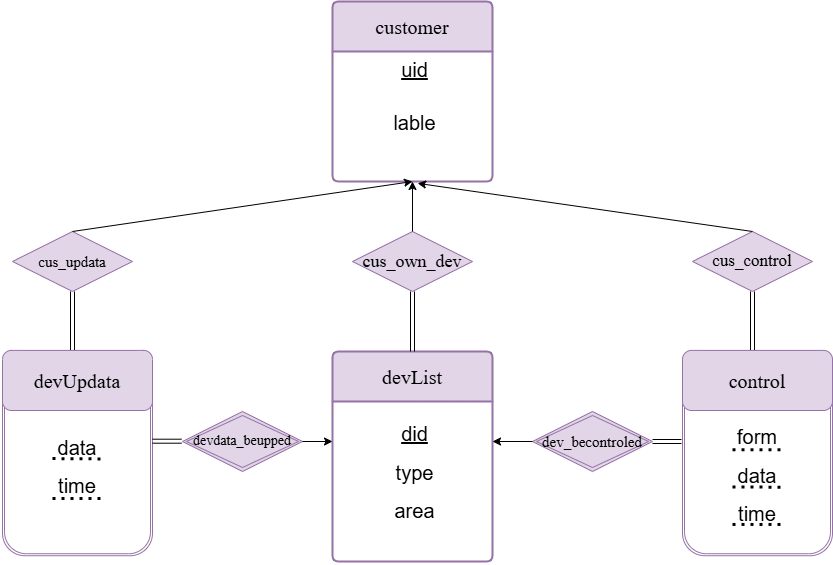
\includegraphics[width=0.48\textwidth]{article/design/figures/smart_home_ER.png}} % 靠左,限制宽度
  \caption{智能家居E-R图}
  \label{fig:smart_home_ER}
\end{figure}

{\begin{CJK*}{UTF8}{zhhei}\subsection{智能家居数据库逻辑设计}\end{CJK*}}

数据库逻辑设计是指在设计数据库结构时,定义表、列、关系和约束等元素的过程。它的目标是根据应用程序需求和数据关系,合理地组织和规划数据库的结构,以实现数据的有效存储、检索和管理。根据上文的智能家居E-R图,将E-R图转化为关系模式,各表的表结构如下:

\begin{enumerate}

    \item 基本信息表:
    
基本信息表也可称为静态信息类表,用于保存智能家居系统中家庭账户信息,智能家居设备信息。基本信息共有两张表:家居账号信息表(customer)与账号设备列表(devList),如下表所示:
    \begin{table}[H]
    \centering
    \caption{家居账号信息表(customer)}
    \vspace{2mm}
    \small
    \begin{tabular}{lllllp{2cm}}
    \toprule
        \textbf{属性} & \textbf{数据类型} & \textbf{长度} & \textbf{主键} & \textbf{外键} & \textbf{含义解释} \\
        \hline
        uid & VARCHAR & 35 & Y & N & 账号id,唯一标识一个账号 \\
        label & INTEGER & 1 & N & N & 使用场景 \\
        \bottomrule
    \end{tabular}
    \label{tab1}
    \end{table}
    \begin{table}[H]
    \centering
    \caption{账号设备列表(devList)}
    \vspace{2mm}
    \small
    \begin{tabular}{lllllp{2cm}}
    \toprule
        \textbf{属性} & \textbf{数据类型} & \textbf{长度} & \textbf{主键} & \textbf{外键} & \textbf{含义解释} \\
        \hline
        uid & VARCHAR & 35 & N & Y & 账号id,唯一标识一个账号 \\
        did & VARCHAR & 35 & Y & N & 设备id \\
        type & VARCHAR & 4 & N & N & 设备型号 \\
        area & VARCHAR & 20 & N & N & 设备房间标签 \\
        \bottomrule
    \end{tabular}
    \label{tab1}
    \end{table}
    \item 实时动态信息表:
    
动态信息表用于记录智能家居中账户对各种家电智能设备的操控监测数据以及设备状态上传信息。实时动态信息一共有两张表:控制操作日志(control)、设备上传日志(devUpdata),如下表所示:
    \begin{table}[H]
    \centering
    \caption{控制操作日志(control)}
    \vspace{2mm}
    \small
    \begin{tabular}{lllllp{2cm}}
    \toprule
        \textbf{属性} & \textbf{数据类型} & \textbf{长度} & \textbf{主键} & \textbf{外键} & \textbf{含义解释} \\
        \hline
        uid & VARCHAR & 35 & N & Y & 账号id,唯一标识一个账号 \\
        did & VARCHAR & 35 & Y & Y & 控制的设备id \\
        time & TIMESTAMP & 20 & Y & N & 控制时间 \\
        form & VARCHAR & 15 & Y & N & 控制方式 \\
        data & VARCHAR & 20 & Y & N & 从远程对设备下发的控制日志 \\
        \bottomrule
    \end{tabular}
    \label{tab1}
    \end{table}
    \begin{table}[H]
    \centering
    \caption{设备上传日志(devUpdata)}
    \vspace{2mm}
    \small
    \begin{tabular}{lllllp{2cm}}
    \toprule
        \textbf{属性} & \textbf{数据类型} & \textbf{长度} & \textbf{主键} & \textbf{外键} & \textbf{含义解释} \\
        \hline
        uid & VARCHAR & 35 & N & Y & 账号id,唯一标识一个账号 \\
        did & VARCHAR & 35 & Y & Y & 上报的设备id \\
        time & TIMESTAMP & 20 & Y & N & 上报时间 \\
        data & VARCHAR & 20 & Y & N & 设备上报的状态日志 \\
        \bottomrule
    \end{tabular}
    \label{tab1}
    \end{table}


\end{enumerate}
\end{CJK*}

